%!TEX root = ../prace.tex

\chapter{Programátorská dokumentace}


%!TEX root = ../../prace.tex

\section{Struktura kódu}
\label{sec:struct}

Protože jsme zvolili implementaci práce v~\UE{}, můžeme využít toho, že engine umožňuje rozdělit celý herní projekt do jednotlivých herních modulů~\citep{epicGameplayModules}. Tím docílíme modularity, nebudeme mít celý projekt v~jednom kuse a~zároveň tím urychlíme překlad projektu při kompilaci.\\
Každý \UE{} projekt musí definovat právě jeden primární herní modul. Pokud využijeme možnosti vytvoření nového projektu založeného na \CPP{}, editor tento modul automaticky vytvoří za nás. My jsme pojmenovali náš projekt {\tt TauCetiF2} a~tak se jmenuje i~náš primární modul.

Jednotlivé části projektu jsme rozdělili do několika herních modulů:

\begin{enumerate}
	\item TauCetiF2 (primární modul)
	\item Inventory
	\item Blocks
	\item Game Save
	\item Commons
\end{enumerate}

Herní moduly jsme seřadili dle jejich závislosti tak, že každý modul závisí na všech modulech s~vyšším očíslováním. Tedy primární modul využívá všech ostatních modulů a~poslední modul (Commons) není závislý na žádném dalším modulu. Pro lepší představu můžeme tyto souvislosti vyjádřit obrázkem \ref{fig:obrStruktura_DependencyDiag}: 

\begin{figure}[!ht]\centering
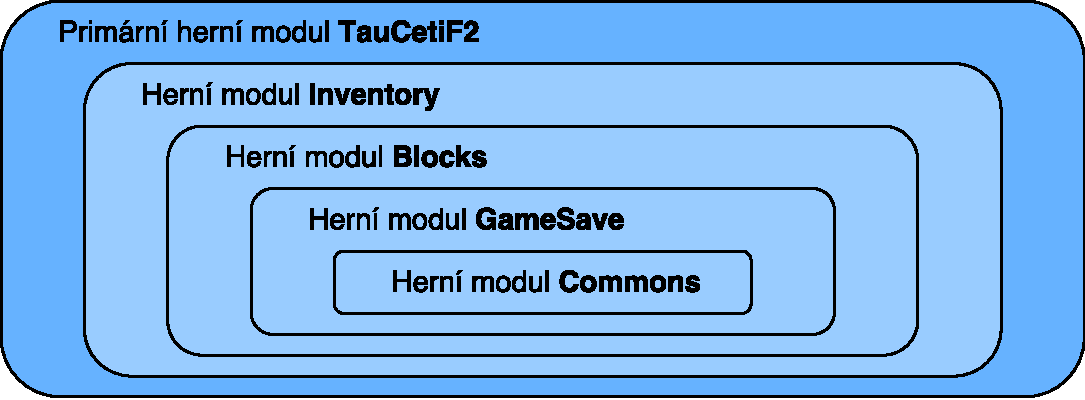
\includegraphics[ width=140mm]{../img/dependencyDiagram}

\caption{Diagram závislostí modulů projektu.}
\label{fig:obrStruktura_DependencyDiag}

\end{figure}

\FloatBarrier

Obecnou koncepci programu jsme popsali v~kapitole \ref{sec:ueStructure}. Abychom se vyhnuli velkému množství dopředných referencí, strukturu programu z~pohledu \CPP{} budeme popisovat od nejnižších vrstev.

\subsection{Obecná struktura modulu}
Všechny moduly dodržují společnou strukturu. Obsahují:
\begin{itemize}
	\item složku \verb!Public!
	\item složku \verb!Private!
	\item soubor \verb![název_modulu].Build.cs!
	\item soubory \verb![název_modulu].h!, \verb![název_modulu].cpp!
\end{itemize}


Každý modul pak má hlavičkové soubory ve složce \TT{Public}, implementaci tříd pak ve složce \TT{Private}. Soubor \TT{*.Build.cs} je využíván nástrojem \UBT{}, zbylé dva soubory definují herní modul v~rámci \UEu{}.




%!TEX root = ../prace.tex

\section{Modul Commons (C++)}

Tento modul je základním modulem, který na jednom místě definuje všechny potřebné informace, které využívají ostatní moduly. Jedná se zejména o definici herních konstant, či definice všech sdílených enumerátorů. Najdeme zde také prapředka použité herní instance. Tuto vlastní implementaci herní instanci využijeme pro ukládání nalezených bloků.

\subsection{Herní definice a konstanty}

\TT{GameDefinitions.h}

Tady jsou definovány všechny herní konstanty. Například je zde definována velikost jednotkové krychle, velikost použitého světa, vztah mezi délkou dne herního světa a počtem uplynulých reálných sekund, převody mezi energií, kyslíkem, zdraví a jednotkou zásahu kyselého deště. Taktéž jsou zde definovány konstanty, které využívá technika obrysů objektu (todo link na outline). Dále jsou zde definovány konstanty ID implementovaných bloků, abychom s nimi mohli pracovat i v kódu.

\subsection{Herní instance}
\TT{TCF2GameInstance.h}

Tato třída je Singleton ( TODO link UE docs) a jako jediná zůstává vždy stejná po celou dobu běhu hry. Proto se využívá například pro uchovávání dat při přechodu mezi jednotlivými Levely a my toho také využijeme. Zároveň se tato třída dá využít pro implementaci delegátů, kterými je možné vyvolat nějakou událost a libovolný prvek z herního světa může tuto událost obsloužit. My toho využijeme u reakce na denní cyklus u bloku \textit{Přepínače}.

Dalším důležitým bodem pro nás bude, že tato třída si bude držet referenci na všechny nalezené bloky. Z předchozího textu již víme, že bloky je potenciálně možné rozšířit o DLC (TODO budem to tu řešit?), takže je nutné, abychom si nalezené bloky a jejich definice udrželi v paměti i při přechodu mezi levely. K tomu slouží proměnná \TT{BlockHolder} , která sice  drží referenci na objekt definovaný v modulu \textit{Blocks}, ale kvůli zpětným referencím mezi moduly (které nejsou povolené) musíme zde použít dostupného předka.

Kód tedy bude vypadat následovně:
\begin{code}
	UPROPERTY(Transient)
		UObject* BlockHolder;

	UFUNCTION(BlueprintCallable, Category = "TCF2 | GameInstance")
		void SetHolderInstance(UObject* holder);
\end{code}
 Parametr \TT{Transient} u makra \TT{UPROPERTY} znamená, že daná proměnná bude vždy nastavena na svoji výchozí hodnotu. V tomto případě je to použito spíše z důvodu zachování konzistence napříč projektu, ale zjednodušeně bychom důsledky mohli popsat následovně -- pokud bude nějaký Blueprint dědit z nějaké \CPP{} třídy, tak vývojář může nastavit výchozí hodnoty properties. Tyto hodnoty jsou pak serializovány do CDO (TODO link?). Během procesu vytváření nové instance objektu, který vychází z daného Blueprintu pak budou tyto hodnoty naplněny během fáze inicializace properties (TODO link na Actor life time?). V konečném důsledku by pak byla tato hodnota nějakým způsobem naplněna. Pokud chceme vynutit, aby tato property nebyla serializována do CDO, tak ji označíme jako \TT{Transient}.

Holder pro nalezené bloky (TODO popsat proč)

\subsection{Enumerátory}

\TT{Enums.h}

co tam je (vypsat všechny, nebo jenom řáct, že je to definované zde, protože je to pro celý projekt?)

\subsection{FFileVisitor}

Kvůli nalezení savů
TODO link na systém ukládání.

\subsection{Helpery}

helpery pro načítání / ukládání konfigurace (vlastních polí)

popsat že UE má mechanismus automatického ukládání vlastností do konfiguračníh souborů, ale to nám nevyhovovalo
%!TEX root = ../../prace.tex

\section{Modul Game Save (C++)}

Modul GameSave slouží k~ukládání a~načítání informací o~probíhající hře do binárního formátu. K~tomu používáme streamové operátory $<<$, které jsou v~tomto případě implementovány tak, že je možné je použít jak pro ukládání, tak pro načítání. // TODO link na tutorial

Díky tomuto přístupu tak můžeme definovat celou strukturu výsledného binárního souboru na jednom místě a~tedy rozšiřování uložené hry je triviální. Co si ovšem musíme pohlídat je to, abychom si drželi informaci o~verzi uloženého souboru. V~našem případě, pokud se bude lišit verze načteného souboru a~uložená konstanta v~programu, save prostě odmítneme (a dokonce smažeme). V~produkčním prostředí bychom si mazání nemohli dovolit, ale museli bychom save ignorovat a~uživateli zobrazit nějakou hlášku o~tom, že verze souboru není podporovaná. My jsme se však v~tomto případě rozhodli save mazat, protože jsme očekávali, že během vývoje hry se bude binární struktura savu často rozšiřovat. Po každé iteraci jsme si savy prostě vytvořili nové.

Zamysleme se nad tím, co by se stalo, kdybychom se snažili načíst save jiné verze. Celá hra by nejspíše byla ukončena s~chybou, protože by se pokoušela číst neplatná data a/nebo by očekávala nějaká data tam, kde žádná nejsou. Tím bychom četli z~neplatné lokace.




\subsection{GameSaveInterface}

\TT{UGameSaveInterface.h} 
Tento soubor definuje rozhraní, které je možné implementovat a~používat v~Blueprintech (struktura vychází z~tutoriálu na Unreal Engine Wiki~\citep{ue_interfaces_tut}). Rozhraní definuje dvě veřejné metody, které musí actoři v~UE při implementaci tohoto rozhraní implementovat:

\begin{code}
UFUNCTION(BlueprintNativeEvent, BlueprintCallable, ... )
	bool SaveGame();

UFUNCTION(BlueprintNativeEvent, BlueprintCallable, ... )
	bool LoadGame();
\end{code}

Hlavní Blueprint levelu pak během svého běhu určité actory přetypuje na tento interface a~bude s~nimi dále pracovat. Podrobněji tato funkcionalita bude popsána v~Blueprintové části.

\subsection{FFileVisitor}

\TT{FFileVisitor.h}

Tento soubor obsahuje implementaci návrhového vzoru Visitor pro získání všech herních savů z~nějaké zadané složky. Implementace vychází z~internetové diskuse na téma procházení adresářů~\citep{ue_iterate_dir}.

\subsection{Helpers}

\TT{SaveHelpers.h}
Tento soubor řeší získání seznamu všech uložených her a~využívá k~tomu implementaci FileVisitoru z~předchozí části.

\subsection{Kontejner s~uloženou hrou}
\TT{SaveGameCarrier.h} Tato třída je v~zásadě přepravkou pro data s~možností ukládání a~načítání dat do binárního formátu. Navíc umožňuje během ukládání v~době vývoje vypsat vlastnosti právě ukládané hry do konzole tak, abychom mohli během vývoje snadno tento výstup zkopírovat a~vytvořit pevně implementované hry. Tyto pevně implementované hry pak nebudou data vracet po přečtení nějakého binárního souboru, ale budou vracet pevně nastavená data. Vytváření těchto pevně vytvořených her pak bylo o~dost jednodušší.

Přepravka obsahuje pouze holá data, tedy nevytvářejí se žádné nové instance herních objektů. To je z~toho důvodu, že nemůžeme použít následující kód:

\begin{code}

// vlastnost kontejneru
TArray<UBlockInfo> UsedBlocks;

// během ukládání
void USaveGameCarrier::SaveLoadData(
	FArchive& Ar,
	USaveGameCarrier& carrier,
	TArray<FText>& errorList,
	bool bFullObject)
{
	Ar << carrier.UsedBlocks;
}
\end{code}
Museli bychom mít referenci na datový typ \TT{UBlockInfo}, který je ale definovaný v~modulu Blocks, který musí nutně modul GameSave referencovat. Tudíž zde použijeme následující konstrukci:

\begin{code}
// vlastnost kontejneru
TArray<FBlockInfo> usedBlocks;

// během ukládání
void USaveGameCarrier::SaveLoadData(
	FArchive& Ar,
	USaveGameCarrier& carrier,
	TArray<FText>& errorList,
	bool bFullObject)
{
	Ar << carrier.usedBlocks;
}
\end{code}

Třídu dědící z~UObjektu jsme nahradili strukturou \TT{FBlockInfo}, která sama slouží pouze jako přepravka na data. Vyšší vrstva, tedy modul Blocks si těmito daty naplní své vlastní objekty, které se pak dále využívají ve hře. A~naopak, před samotným uložením se postará o~to, aby bylo toto pole korektně naplněno všemi daty určenými k~uložení. O~samotnou serializaci a~deserializaci dat do a~z~přepravky se stará pouze modul GameSave.

Celý systém vychází z~tutoriálu~\citep{ue_save_system} je postaven na tom, že v~C++ je možné přetěžovat operátory, mimo jiné i~$<<$. Této vlastnosti je využito tak šikovně, že v~závislosti na volání funkce buď zapisuje do archivu, nebo z~něj čte, ale pořád se jedná o~jediný zápis jedné funkce. To je výhodné, protože to předchází chybám, které by mohly vzniknout při použití 2 metod -- jedné čtecí, jedné zapisovací. Chybám typu přehození dvou datových typů (což by v~případě typů různých velikostí znamenalo následné špatné pochopení binárních dat), nebo kupříkladu prohození dvou vlastností stejného typu, což by vytvářelo těžko odhalitelné situace změn hodnot ve hře.

Tento systém je použit pro všechny rozšířené části herního savu -- Bloky, Inventář, Počasí -- a~všechny používají podobný způsob práce. Jedná se o~definici struktur, tedy samotných kontejnerů a~dále pak jeden soubor pojmenovaný \TT{*ArchiveHelpers.h}, kde je popsána vlastní struktura daných kontejnerů v~Archivu. Hvězdičku v~tomto případě bereme opravdu jako zástupný symbol. Navíc, některé objekty mohou řídit archivaci dle nějakých podmínek nastavených shora. Příkladem budiž definice serializace elektrické komponenty:

\begin{code}
// přetížení, které se nevolá vždy
FORCEINLINE FArchive& operator<<(
	FArchive &Ar,
	FPoweredBlockInfo& componentInfo)
{
	Ar << componentInfo.IsOn;
	Ar << componentInfo.AutoregulatePower;
	Ar << componentInfo.PowerConsumptionPercent;
	return Ar;
}

FORCEINLINE FArchive& operator<<(
	FArchive &Ar, 
	FElectricityComponentInfo& componentInfo)
{
	Ar << componentInfo.CurrentObjectEnergy;
	Ar << componentInfo.HasPoweredBlockInfo;

	// pokud máme navíc rozšiřující data, přidáme další data
	// tím efektivně zavoláme metodu uvedenou výše
	if (componentInfo.HasPoweredBlockInfo)
		Ar << componentInfo.PoweredBlockInfo;

	return Ar;
}
\end{code}

Jak vidíme z~kódu, celý kód se chová korektně jak při serializaci, tak i~při deserializaci. Je pouze potřeba vzít v~úvahu, že vyšší struktury, které pak budou tyto data používat pro vlastní inicializaci, musí také brát v~potaz podmínku. Pokud není splněna, tak svázaná proměnná (v tomto případě \TT{PoweredBlockInfo}) nebude obsahovat platná data.

\subsection{NewGameSaveHolder}

\TT{NewGameSaveHolder.h} Tato třída je hlavní třídou, se kterou hra před načítáním pracuje. Definuje seznam napevno zabudovaných levelů a~obsahuje jejich implementaci.










%!TEX root = ../prace.tex

\section{Modul Blocks (C++)}

Modul bloků obsahuje podstatné informace o tom, jak hra pracuje s bloky, jak se tyto bloky skládají do herního světa, jaké jsou jejich komponenty apod. Také je v tomto modulu možné nalézt specifické implementace jednotlivých bloků.

V dalším textu se budeme odkazovat na složky. Odkazujeme se tím do složek \TT{/Source/Blocks/Public} a jejich  \TT{Private} implementací. Strukturu bychom mohli shrnout následovně:

\begin{enumerate}
	\item Definice bloků (složka \TT{Definitions})
	\item Třídy s popisem bloků (složka \TT{Info})
	\item Systém ukládání a načítání bloků (složka  \TT{Helpers})
	\item Rozhraní, které mohou bloky implementovat (složka \TT{Interfaces})
	\item Komponenty, kterými bloky rozšiřují svoji základní funkcionalitu (složka \TT{Components})
	\item Implementace jednotlivých bloků (složky \TT{BaseShapes}, \TT{Special})
	\item Stromové struktury herního světa (složka \TT{Tree})
\end{enumerate}
 

\subsection{Definice bloků}
V této složce se nachází všechny definiční soubory bloků. Definiční soubor obsahuje pouze popis datové struktury a nějakou minimální funkcionalitu (kupříkladu získání korektního vektoru velikosti v závislosti na tom, zda má definice daného bloku nastavenou vlastní velikost). Jednotlivé konkrétní instance s daty jsou pak definovány na straně editoru. Konstanty (například minimální a maximální škálování) je pak možné měnit v editoru a není vyžadována rekompilace projektu hry. 

Definiční soubor se skládá následujícím způsobem:

\begin{itemize}
	\item UBlockDefinition (\TT{BlockDefinition.h})
		\subitem -- FUsableBlockDefinition (\TT{UsableBlockDefinition.h})
		\subitem -- FBlockMeshStructureDefinition (\TT{BlockMeshStructureDefinition.h})
			\subsubitem -- FBlockMaterialDefinition (\TT{BlockMaterialDefinition.h})
		\subitem -- FBlockAdditionalFlags (\TT{BlockAdditionalFlags.h})
			\subsubitem -- FBlockFlagValue (\TT{BlockFlagValue.h})	
		\subitem -- FOxygenComponentDefinition (\TT{OxygenComponentDefinition.h})
		\subitem -- FElectricityComponentDefinition (\TT{ElectricityComponentDefinition.h})
			\subsubitem -- FElectricityBindableAreas (\TT{ElectricityBindableAreas.h})	
				
		

\end{itemize}

\subsection{Třídy s popisem bloků}
Tyto třídy popisují už konkrétní instance bloků v rámci hry. Jejich hodnoty jsou pak v mezích definovaných v definičních třídách. Tyto třídy jsou pak předmětem ukládání a načítání. Dalším důležitým prvkem je BlockHolder, který slouží pro nalezení bloků. 

\subsection{Ukládání a načítání bloků}

- ukládání - máme něco jako block saving helpers


\subsection{Interfaces}
poskytují nástroje pro volání metod na instaních interfacu

popsat ideu za Implementation, Execute (BlueprintNativeEvent, BlueprintImplementableEvent)

\subsection{Komponenty bloků}
- pak máme komponenty bloků a nějaké interfaces

\subsubsection{Elektrická komponenta}


\subsubsection{Elektrická síť}


\subsubsection{Kyslíková komponenta}


\subsubsection{Select target}


\subsubsection{World object}






\subsection{Implementace bloků}
 - základ Block.h, zbytek v jendotlivých podkategoriích (BaseShapes / Special
 
 TODO jak moc podrobné? vypsat všechny bloky a co všechno implementují, nebo to stačí stručně zmínit? - co implementují by si čtenář mohl uvědomit z předchozího textu a navíc je to jen nudný popis, jehož výžpovědní hodnota je ve zdrojácích a není asi nutné to tu duplikovat

- popsat speciální bloky + nějaké speciality co umějí (showableWidget)


\subsection{Stromové struktury}
popsat stromové struktury, které tam mám


\subsubsection{MinMaxBox}

prapředek všeho



\subsubsection{KDTree}

dědí z MMB, základ ve světě


\subsubsection{WeatherTargetsKDTree}

dědí z MMB, slouží pro potřeby počasí
%!TEX root = ../prace.tex



\section{Modul Inventory (C++)}

Modul inventáře byl vyčleněn do samostatné části. Je to hlavně jako ukázka možného členění do modulů. Navíc časem by se mohl tento modul rozšířovat jak by rostla kompelxicita správy inventáře.

Nejdůležitější inventory component


\subsection{Tag group}
nejnižší úroveň, odpovídá 'nebo'

\subsection{Inventory tag group}

celá skupina, odpovídá 'A zároveň'

\subsection{Inventory tags}

sdružuje všechny banky

\subsection{Inventory component}

celá komponenta, která je pak navázaná na hráčův charakter

definuje delegáty notifikující o změnách v akivní skupině, po filtrování apod.

na této úrovni se řeší aktualizace cache buildable i inventorybuildable při změnách, zároveň poskytuje možnost clear cache pro volání shora (BP)


%!TEX root = ../prace.tex

\section{Modul TauCetiF2 (C++)}
- primární modul

popsat co všechno obsahuje (widgety, gamemodes, weather apod)

- popsat synchronize widget ( // TODO link na důvod, proč to tam mám), popsat object widget, napsat důvody

- popsat to stackování 

- popsat komponenty
(weather, game electricity)







\chapter{Backlog}

Zde popsat jak jsem to celé implementoval a proč\\

Popsat jednotlivé moduly a nakreslit diagram vztahů mezi nimi\\

Popsat strukturu save gamu + důvod proč jsem to tak udělal
+popsat načíttání savů + systémových savů


Popsat jednotlivé C++ třídy a jejich odvozené Blueprintové deriváty + přidat případné obrázky z BL kódu (např. BlueprintImplementable event, který se zavolá jak na C++ tak i na BP) \\

Udělat rozbor BT počasí + mechaniku počasí + denního cyklu
popsat řízení osvětlení dle počasí

Udělat rozbor bloků, škálování, konfigurace, datovou strukturu, implementaci dynamických textur, zvýraznění

Popsat mechaniku Selector - SelectTarget + napojení na Builder

Popsat mechaniku používání objektů + zvýraznění

Popsat mechaniku Inventáře

// TODO vymyslet vhodné pořadí, abych neskákal mezi prvky, toto pořadí dodržet i v předchozích kapitolách

-> Mám svět, ten má v sobě bloky, ty jsou v nějaké stromové struktuře, bloky mají komponenty, které přes tuto strukturu mohou na sebe vázat
Svět má také počasí se svojí vlastní strukturou, vuyžívající podobnosti s bloky (2D KD strom s Heapem na listech)

-> hráč může to a tamto, díky inventáři se dostane na bloky, a díky selectoru je pak můževložit do světa skrz World controller (zmíněno v předchozím)
->zároveň jsou všechny entity savovatelné 


-> Popsat struktury Widgetů, zmínit použití Synchronize Widgetu, implementaci mechaniky stackovatelných widgetů

-> popsat implementaci hudby

-> TODO otestovat možnost nového bloku v rámci DLC
->Zmínit zároveň, že s tímto by šlo tweakovat nastavení hry



// TODO obrázky s konfiguračními ukázkami do příloh (např. jak se definuje Blok z UE


